\chapter{Generating Test Cases}\label{ch:tests}

In this chapter, we show how to use occurrence graph grammars to generate test cases and oracles from (simply-typed) graph grammars that model systems. In theory, this approach can be used to generate tests for any graph grammar, since it is based only on the properties of the formalism. However, we focused on graph grammars that were generated from use cases by using the methodology presented in \cite{Junior2015}, \cite{BezerraWEIT2016} and \cite{Cota2017}.

This methodology is a systematic, computer-aided way to extract graph grammars from use cases or other text-based requirement documents. At the same time, it helps finding problems such as ambiguities, inconsistencies and omissions in the documents. Thus, providing a better specification and also an improved model.

Following from there, by generating tests from these grammars we are indirectly generating tests from their (verified) use cases. The test generation, to be described in next sections, was implemented in verigraph as an extension to the calculation of the occurrence graph grammars that were previously discussed. 

Basically, we are interested in knowing whether each functionality of a system is truly executable, i.e. whether all the rules that represent each functionality flow are applicable.

If it happens that a functionality is not executable, we want to know exactly what is the problem that is preventing its execution. On the other hand, if it is executable, we are interested in:

\begin{enumerate}
\item the input data necessary for this functionality to execute, as well as the output data of a successful execution;

\item at least one path (for each flow) in which the rules can be applied to accomplish the functionality goals;

\item a set of constraints which can tell the test analyst how two characterize the tests into those which should pass and those which should fail;

\item a set of constraints which can tell which intermediate states of the system are valid and those that are not.
\end{enumerate}

Notice that the two first items correspond to test cases while the other two correspond to test oracles.

%First, we present a brief overview of the methodology for extracting graph grammars from use cases, after what we present the process of generating the tests cases from the extracted grammars.

\section{Overview of the extracting methodology}

Usually, use case documents consist of sets of sequential steps describing the interaction between an actor and a system in order to accomplish a specific goal. In general, one of these sets represents a successful (normal or main) execution of the system, whereas other sets represent sequences of alternative or exception flows. Moreover, use cases may also contain pre- and post-conditions used to indicate the configurations that must hold before and after their execution.

Figure~\ref{fig:tests:methodology} summarizes the methodology process proposed in \cite{Junior2015}, showing how to extract a graph grammar from a text-based requirements document. This methodology is divided into four main phases:

\begin{description}
  \item[Data Extraction:] identification of entities and actions that will be used to construct the model.

  \item[Primary Verifications:] checking for problems that might affect or prevent the creation of the model, as well as the removal of this problems from the use case. Some examples are:entities or conditions are listed but are never used or effects of actions that are not clearly defined.

  \item[GT Generation:] construction of graph transformation model by modelling conditions and effects as graphs, building a type graph and then modelling each step of the use case as a transition rule from one state graph to another.

  \item[UC Analysis:] automated verifications over the model in order to detect possible flaws in the use case. This is step is done using verigraph and its concurrent rules, conflict and dependency analyses.
\end{description}

We use a grammar that models an e-store system in our example. This grammar was extracted, using the methodology, from a set of use cases presented in~\cite{Goins2007}. These use cases model basic e-store functionalities such as \emph{browse catalogue, user registration, login, update user information, maintain shopping cart}, among others.

Some excerpts of this grammar are shown throughout this chapter, while the complete extracted grammar can be found on appendix~\ref{app:marvel-grammar} and at the Verites repository for case studies\footnote{https://github.com/Verites/case-studies}.

\begin{figure}[!ht]
  \centering
  \fbox{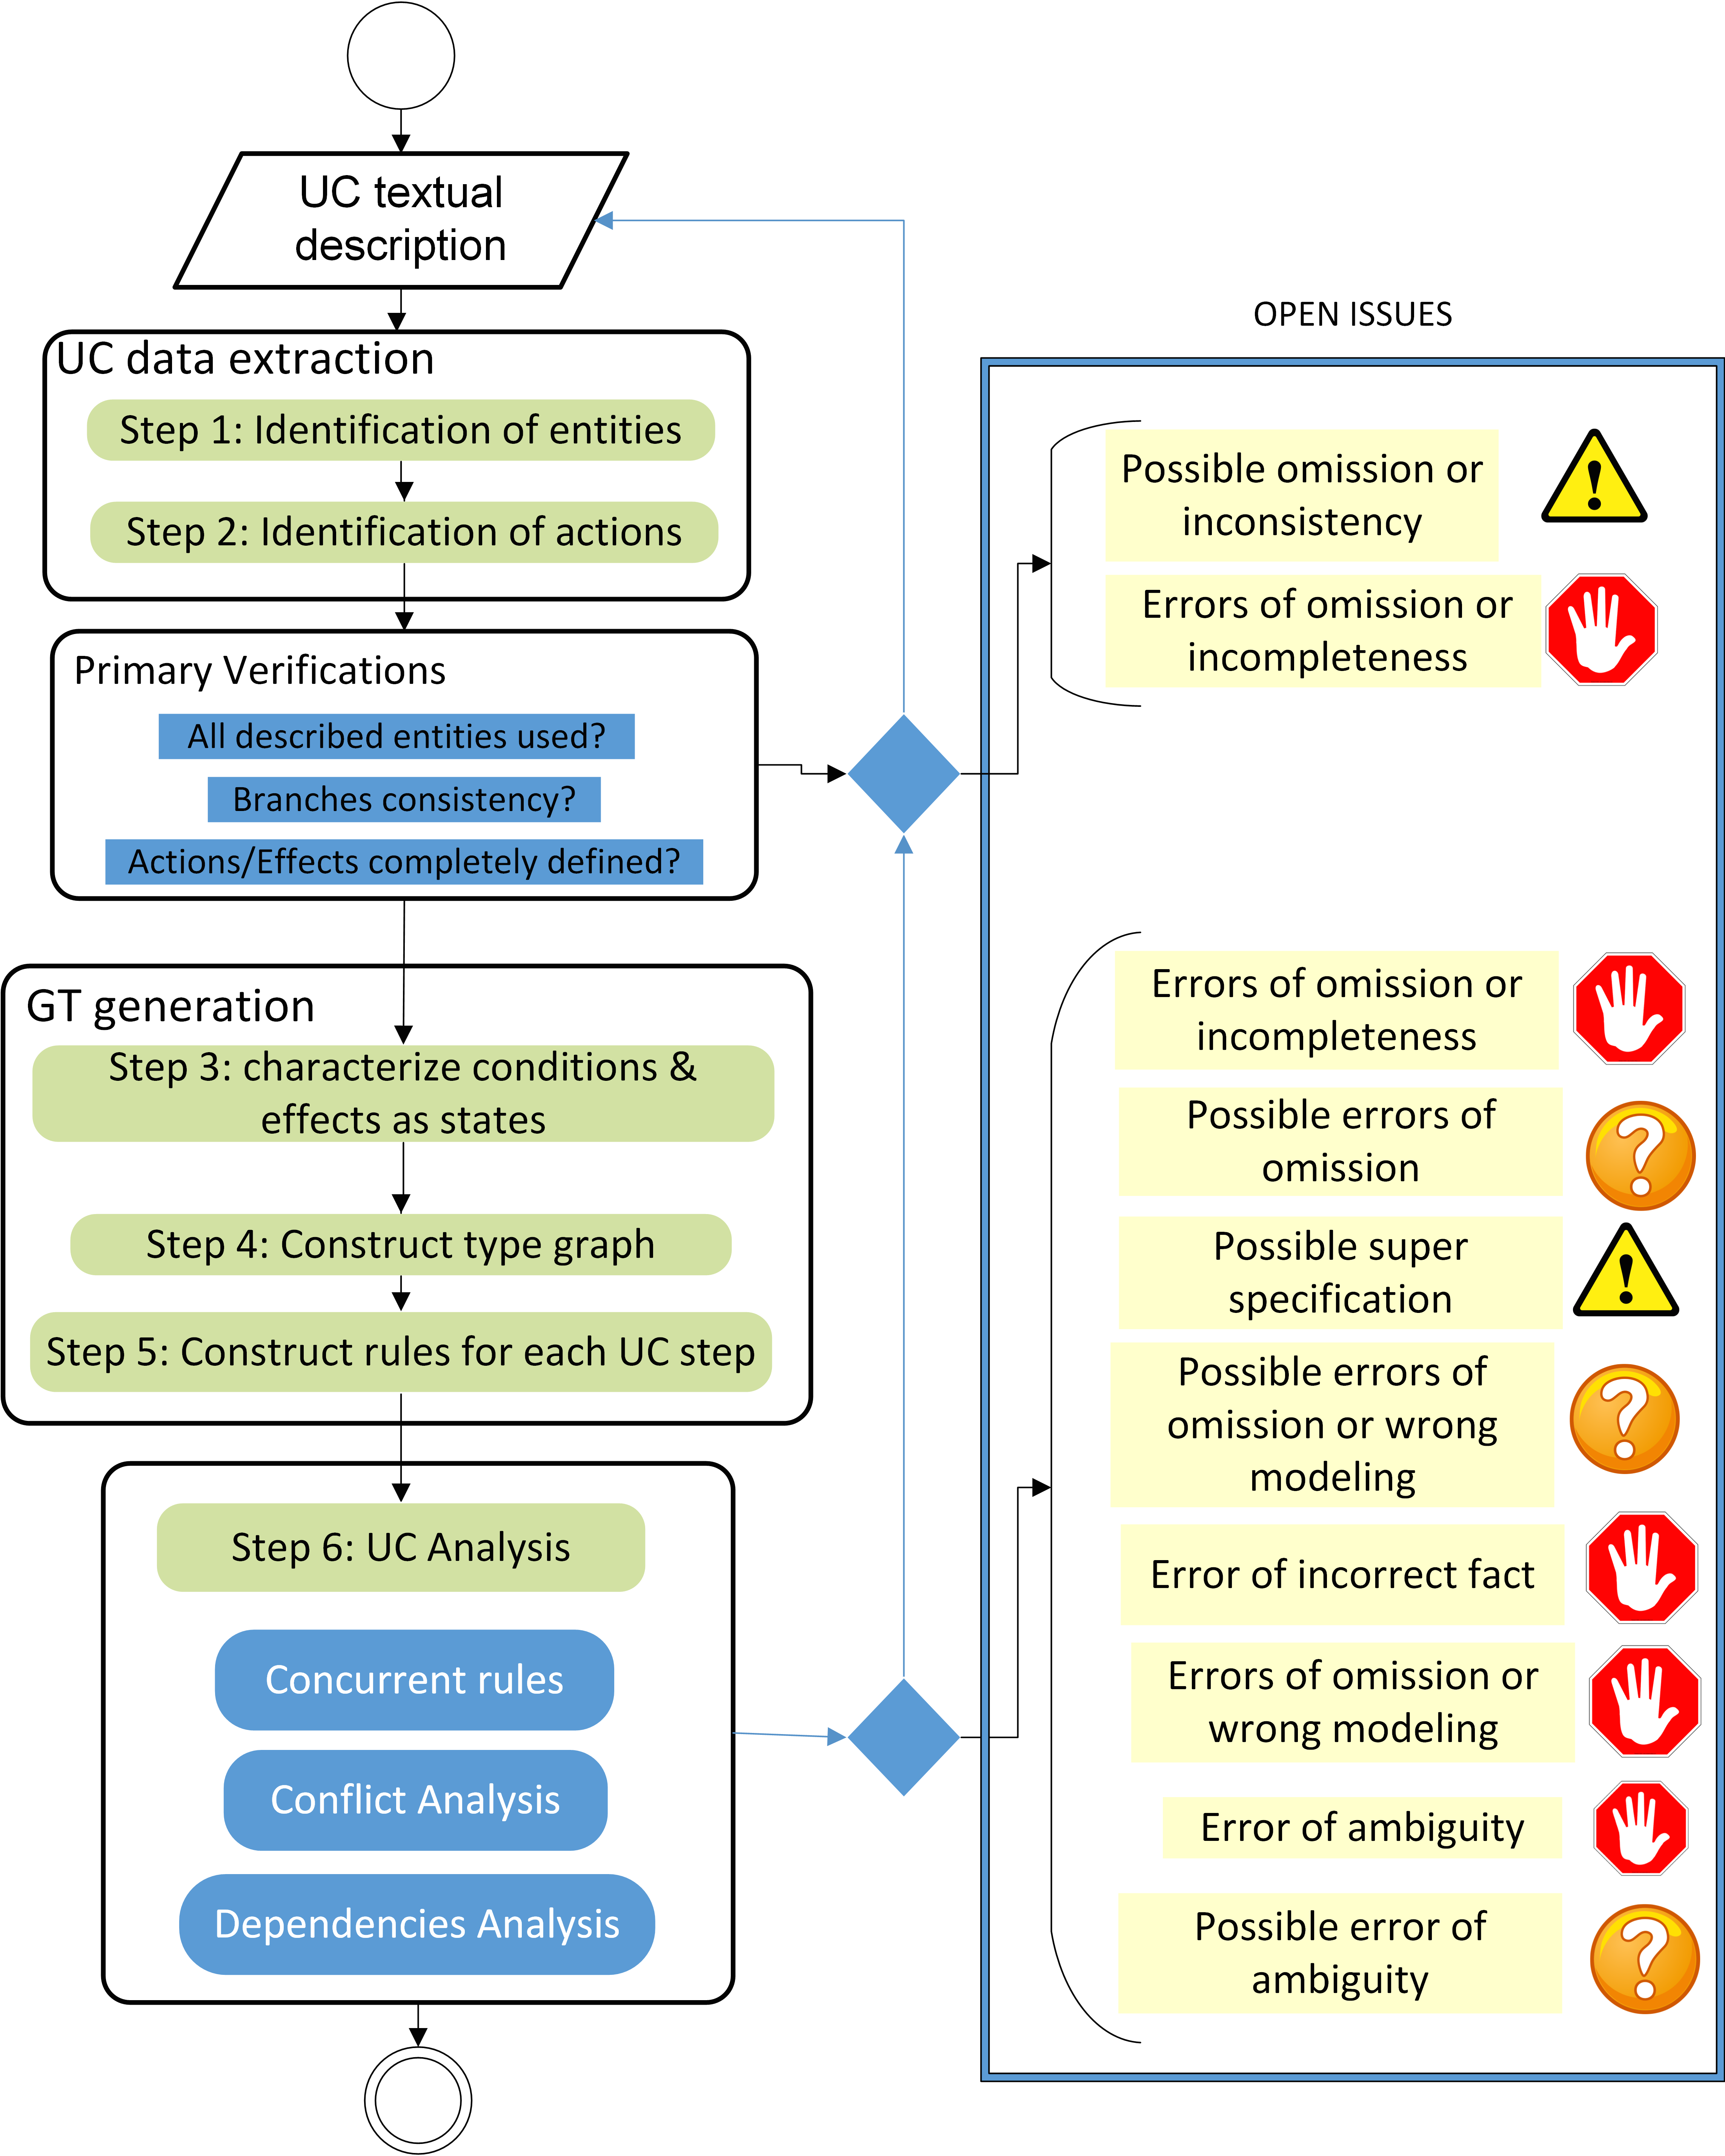
\includegraphics[scale=0.6]{images/generating-tests/methodology}}
  \caption{Overview of the methodology~\cite{Junior2015}.}\label{fig:tests:methodology}
\end{figure}

\section{Generating Tests using Occurrence Graph Grammars}

Given a graph grammar \graphGrammar{} that models a system, we want to generate test cases and oracles for each subset of rules $F_i \subseteq P$ $\forall i \in 1\ldots n$, where $F_i$ represents a complete functionality \tinytodo{feature} of the system.

\begin{example} Figure~\ref{fig:tests:grammar} we show a subset of the rules from the e-store grammar that represents the use case \emph{browse catalogue}. 

\begin{figure}[!ht]
  \centering
  \begin{subfigure}[t]{.5\textwidth}
    \centerline{\fbox{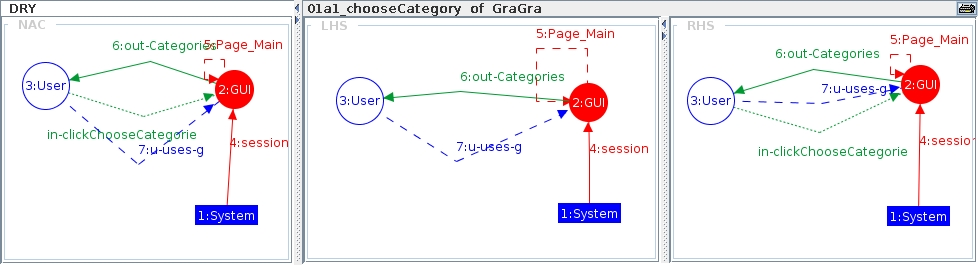
\includegraphics[scale=0.5]{images/generating-tests/grammar/rule01}}}
    \caption{Rule \emph{choose category}}
  \end{subfigure}
  \begin{subfigure}[t]{.5\textwidth}
    \centerline{\fbox{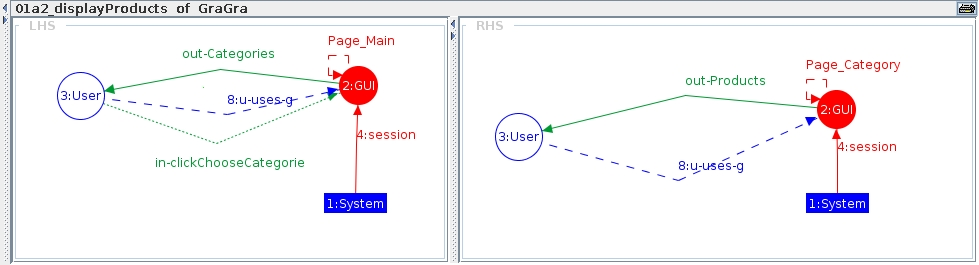
\includegraphics[scale=0.5]{images/generating-tests/grammar/rule02}}}
    \caption{Rule \emph{display products}}
  \end{subfigure}
  \begin{subfigure}[t]{.5\textwidth}
    \centerline{\fbox{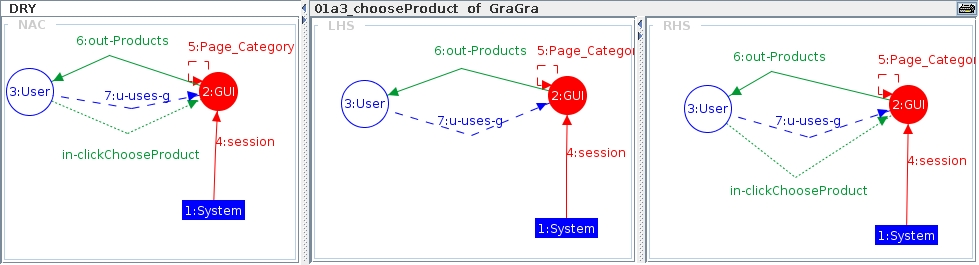
\includegraphics[scale=0.5]{images/generating-tests/grammar/rule03}}}
    \caption{Rule \emph{choose products}}
  \end{subfigure}
  \begin{subfigure}[t]{.5\textwidth}
    \centerline{\fbox{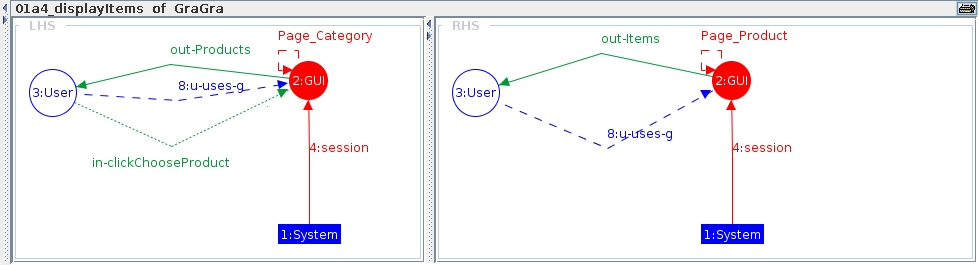
\includegraphics[scale=0.5]{images/generating-tests/grammar/rule04}}}
    \caption{Rule \emph{display items}}
  \end{subfigure}
  \caption{Rules for the use case \emph{browse catalogue}}\label{fig:tests:grammar}
\end{figure}

\begin{figure}[!ht]
\ContinuedFloat
\centering
  \begin{subfigure}[t]{.5\textwidth}
    \centerline{\fbox{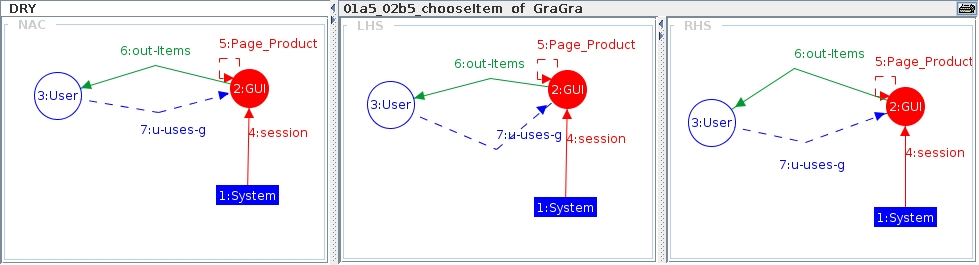
\includegraphics[scale=0.5]{images/generating-tests/grammar/rule05}}}
    \caption{Rule \emph{choose item}}
  \end{subfigure}

  \begin{subfigure}[t]{.5\textwidth}
    \centerline{\fbox{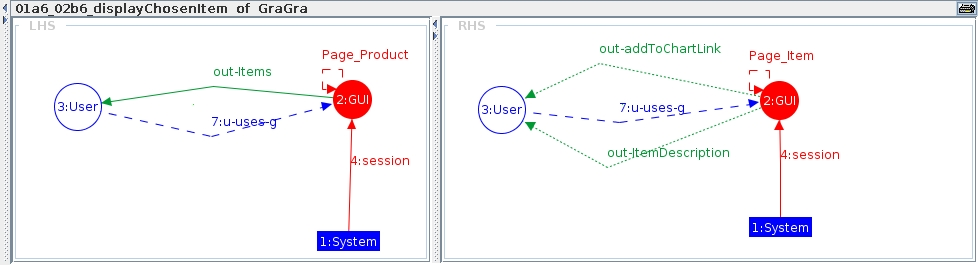
\includegraphics[scale=0.5]{images/generating-tests/grammar/rule06}}}
    \caption{Rule \emph{display chosen item}}
  \end{subfigure}
\end{figure}

\subsection{Preparing the input}

Together with the grammar $GG$ and its subsets of functionalities $F_i$, we will also need an \emph{input-output relation} $IO_i$ for each $F_i$, specifying the connections between the rules in the subsets. This \emph{input-output relation} identifies which elements (nodes and edges) must be the same between each pair of rules, as shown in example~\ref{ex:inout}.


  For this use case we have one main execution path and \tinytodo{number} alternative paths. Thus, we have $n$ features.
  Thus we have the following subsets:
  \begin{itemize}
    \item $F_1 = \{\}$, the main path;
    \item $F_2 = \{\}$, the.
  \end{itemize} \tinytodo{complete}
\end{example}

Once having the sets of rules, we know need to build the input-output relations for each one of them.

\begin{example}[Input-Output Relations]\label{ex:inout} A \emph{full} input output-relation for all rules of a subset has the appearance of the following diagram, where we have a set of $IO$ objects that are nothing more then a graph with a pair of morphism mapping one left-hand side of a rule with the right-hand side of another rule.

\diagram{
  & & & & IO_6\ar@{-->}[dddrrrr]\ar@{-->}[dddllll] & & & &\\
  & IO_3\ar@{-->}[ddl]\ar@{-->}[ddrrrr] & & & & & & IO_4\ar@{-->}[ddr]\ar@{-->}[ddllll] &\\
  & & IO_1\ar@{-->}[d]\ar@{-->}[dr] & & IO_5\ar@{-->}[drr]\ar@{-->}[dll] & & IO_2\ar@{-->}[d]\ar@{-->}[dl] & &\\
  L_1 & K_1\ar[l]\ar[r] & R_1 & L_2 & K_2\ar[l]\ar[r] & R_2 & L_3 & K_3\ar[l]\ar[r] & R_3\\
  }\hfill\break

    Figure~\ref{fig:tests:inout} shows how an $IO$ object connects two different rules, which is similar to how the interface graph of a rule identifies the elements that are the same in its left and right sides.

    For most of the cases, a full relation will not be necessary, as the $IO$ relation has some sort of transitivity. Thus, we can focus on build only a subset of it. For example, in \tinytodo{draw and explain}

\begin{figure}[!ht]
  \centering
  \fbox{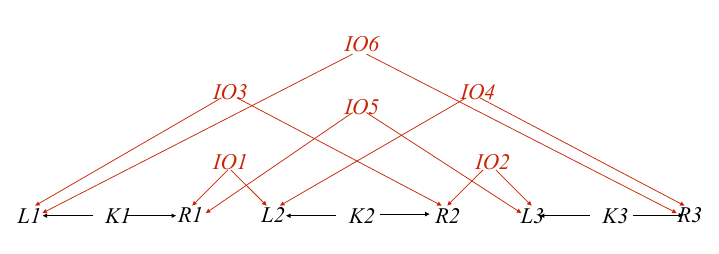
\includegraphics[scale=0.7]{images/generating-tests/inout}}
  \caption{Input-Output relation structure.}\label{fig:tests:inout}
\end{figure}

\end{example}

Now that we have a $GG$ modelling a system, its set of rules $P$, together with $F_i$ and $IO_i$, we generate as output:

\begin{enumerate}
\item an amalgamation (colimit) $OGG_i$ of rules for each $F_i$ with respect to $IO_i$
\item the initial and final graphs $I_i$ and $J_i$ of $OGG_i$, representing the input and output data of the functionality $F_i$
\item the conflict and dependency relations between rules \tinytodo{and the elements involved in the conflict / dependency}
\item restrictions over the ordering of elements existence and rules applicability
\item one or more total orderings that respect all relations and restrictions
%\item one or more total orderings that do not respect the relations or restrictions
\end{enumerate}

First, the amalgamation of rules in $F_i$ w.r.t. $IO_i$ is responsible to ``glue'' the graphs of all rules in on single graph at the same that it identifies the items that come from different rules but are supposed to be the same element.

The colimit of a diagram such as the one presented in Example~\ref{ex:inout} has the following format, where $Occ$ is the amalgamation object, i.e. $Occ$ contains all the concrete elements of the rules where it came from:

\diagram{
  & & & & IO_6\ar[dddrrrr]\ar[dddllll] & & & &\\
  & IO_3\ar[ddl]\ar[ddrrrr] & & & & & & IO_4\ar[ddr]\ar[ddllll] &\\
  & & IO_1\ar[d]\ar[dr] & & IO_5\ar[drr]\ar[dll] & & IO_2\ar[d]\ar[dl] & &\\
  L_1\ar[dddrrrr] & K_1\ar[l]\ar[r] & R_1\ar[dddrr] & L_2\ar[dddr] & K_2\ar[l]\ar[r] & R_2\ar[dddl] & L_3\ar[dddll] & K_3\ar[l]\ar[r] & R_3\ar[dddllll]\\
  & & & & & & & &\\
  & & & & & & & &\\
   & & & & Occ & & & &
}\hfill\break

If the result of this colimit is a \emph{core graph} according to definition~\ref{def:core-graph}, we can create a doubly-typed graph grammar $OGG_i$ that is also a strongly-safe grammar and therefore a candidate to be an occurrence graph grammar.

Remember that, if there is more than one rule that deletes or creates the same element, it is not possible to apply all rules of this functionality, and $OGG_i$ can not be an occurrence graph grammar.

\begin{example}[Amalgamation example]\label{ex:amalgamation} Figure~\ref{fig:tests:colimit} shows the object resultant from the amalgamation of the rules of our running example, presented in Figure~\ref{fig:tests:grammar}.

\begin{figure}[!ht]
  \centering
  \fbox{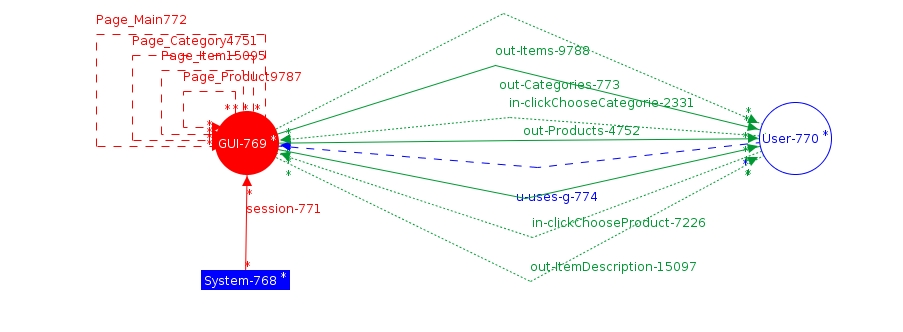
\includegraphics[scale=0.4]{images/generating-tests/colimit}}
  \caption{Amalgamation (colimit) of rules according to the IO relation.}\label{fig:tests:colimit}
\end{figure}

\end{example}

After identifying that $OGG_i$ is in fact a strongly-safe graph grammar, we can extract the initial and final graphs of $OGG_i$ by removing from the core graph the created and deleted elements, respectively. If they are valid graphs, we have the input and output data for the test case. Otherwise, if they have dangling edges, it is not possible to apply all rules of the functionality, since it would begin in or lead to an inconsistent state.

\begin{example}[Initial and Final Graphs Example] Figure~\ref{fig:tests:graphs}.

  Notice that the elements \tinytodo{make list} are created by rules \tinytodo{make list}, and therefore do not appear in the initial graph. Similarly, the elements \tinytodo{make list} are deleted by rules \tinytodo{make list} and do not appear in the final graph.

\begin{figure}[!ht]
  \centering
  \begin{subfigure}[t]{.5\textwidth}
    \centerline{\fbox{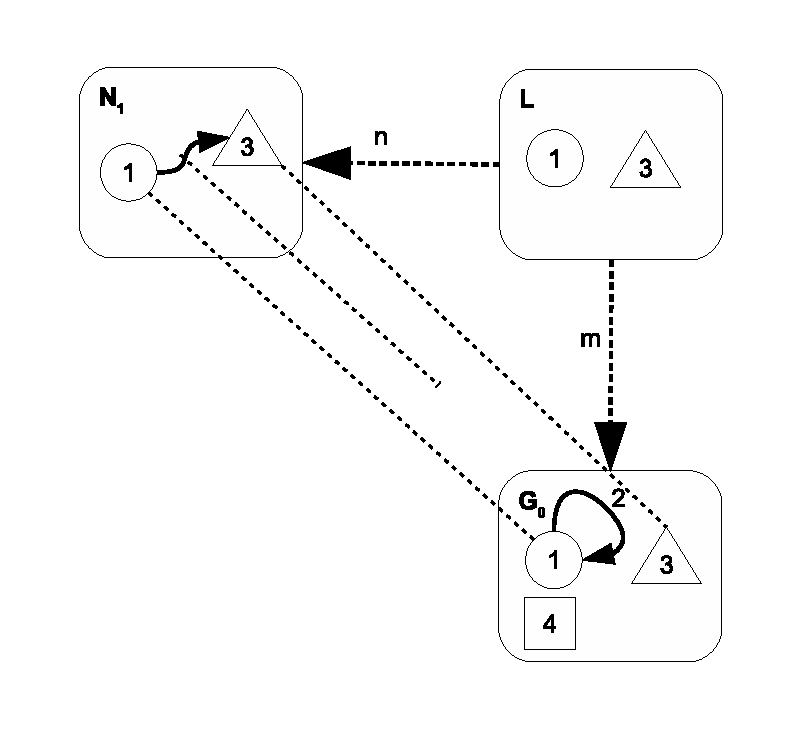
\includegraphics[scale=0.55]{images/gts/satisfied_nac}}}
    \caption{Initial graph}
  \end{subfigure}%
  \begin{subfigure}[t]{.5\textwidth}
    \centerline{\fbox{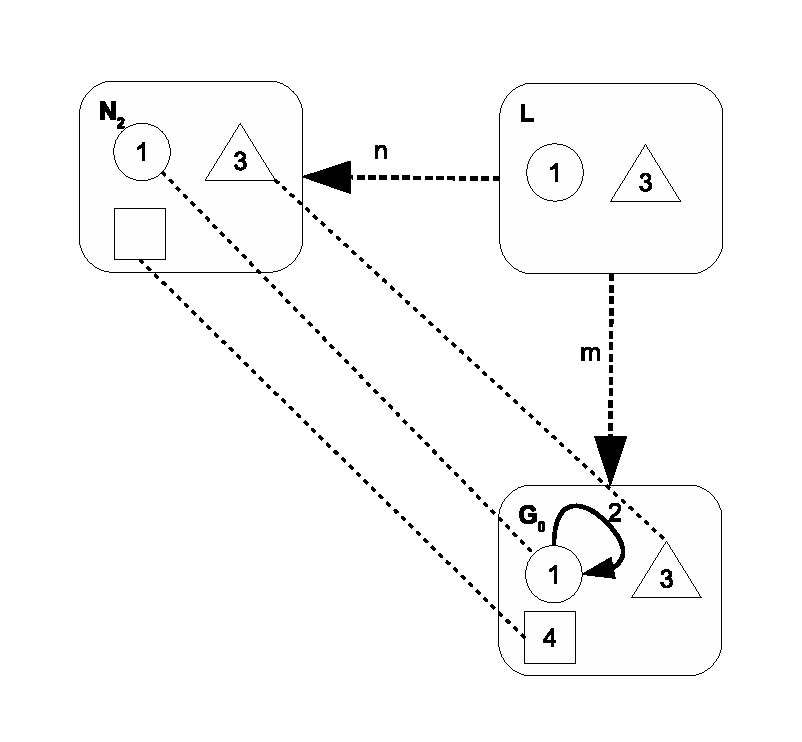
\includegraphics[scale=0.55]{images/gts/triggered_nac}}}
    \caption{Final graph}
  \end{subfigure}
  \caption{Instance graphs}\label{fig:tests:graphs}
\end{figure}
\end{example}

Once the previous verifications were successful, we can build the occurrence relation (and any other relation discussed on chapter~\ref{ch:process}) to verify if $OGG_i$ can really be an occurrence graph grammar. If no abstract dependencies or conflicts are found, then the concrete relations are sufficient to do this verification, thus we simply need to check if there is a total ordering compatible with the relations.

\begin{example}[Occurence Relation]
\end{example}

If the set $R$ of \emph{occurrence relation restrictions} is not empty, we also need to check if there is a total ordering of the occurrence relation that respects these restrictions.

As this seems to be a hard problem, in the complexity sense, we left this last implementation as a future work. However, we still use the restrictions to generate a set of tests regarding the consistency of the system states.

In our case estudies, no such situation was found. We believe that it happens because we used grammars extracted from real use cases, where usually there are (possibly many) sequential connections between the actions, which forces the rules to be connected via the \emph{occurence relation} and avoids abstract restrictions.

\section{Building test cases with Verigraph}

More specific usability details can be found on the Verigraph tutorial, whose current version is presented on appendix~\ref{app:tutorial}.
